%=== Einheit  ====================================================================
\Tut\chapter{Endliche Automaten}
\label{k:endl-auto}

%-----------------------------------------------------------------------
\Tut\section{Erstes Beispiel: ein Getr\"ankeautomat}
\def\mybox#1{\hbox{\vrule height 2ex width 0pt depth 0.6ex#1}}
\def\taste[#1]#2{%
  \tikz[x=8mm,y=8mm,baseline=(N.base)] \tasteinnerx[#1]{#2};%
}
\def\tasteinnerx[#1]#2{%
  \node[midway,inner sep=0mm,draw,rounded corners,anchor=base,minimum width=10mm,#1] (N) {\mybox{#2}}%
}
\def\tasteinner[#1]#2{%
  node[midway,inner sep=0mm,draw,rounded corners,minimum width=10mm,#1] (N) {\mybox{#2}}%
}
\def\tasteinnerOK{\tasteinner[fill=green!20]{OK}}
\def\tasteOK{\taste[fill=green!20]{OK}}
\def\tasteC{\taste[fill=red!20]{C}}
\def\tasteinnerC{\tasteinner[fill=red!20]{C}}
\def\tasteRein{\taste[fill=blue!10]{rein}}
\def\tasteinnerRein{\tasteinner[fill=blue!10]{rein}}
\def\tasteZitro{\taste[fill=yellow!10]{zitro}}
\def\tasteinnerZitro{\tasteinner[fill=yellow!10]{zitro}}

\begin{extract}[tut]
  \begin{itemize}
  \item siehe Skript;
  \end{itemize}
\end{extract}

Als erstes Beispiel betrachten wir den folgenden primitiven
Getränkeautomaten (siehe Abbildung~\ref{fig:getraenkeautomat}).  Man
kann nur 1-Euro"=Stücke einwerfen und vier Tasten drücken: Es gibt
zwei Auswahltasten für Mineralwasser \tasteRein{} und Zitronensprudel
\tasteZitro{}, eine Abbruch"=Taste \tasteC{} und eine \tasteOK-Taste.

\begin{itemize}
\item Jede Flasche Sprudel kostet 1 Euro.
\item Es kann ein Guthaben von 1 Euro gespeichert werden. Wirft man
  weitere Euro"=Stücke ein, werden sie sofort wieder ausgegeben.
\item Wenn man mehrfach Auswahltasten drückt, wird der letzte Wunsch
  gespeichert.
\item Bei Drücken der Abbruch"=Taste wird alles bereits eingeworfenen
  Geld wieder zurückgegeben und kein Getränkewunsch mehr gespeichert.
\item Drücken der OK-Taste wird ignoriert, solange noch kein Euro
  eingeworfen wurde oder keine Getränkesorte ausgewählt wurde.

  Andernfalls wird das gewünschte Getränk ausgeworfen.
\end{itemize}

\begin{figure}[ht]
  \centering
  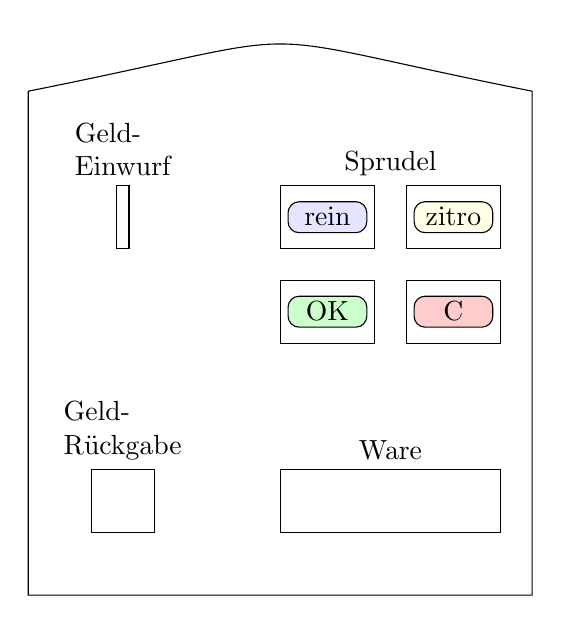
\begin{tikzpicture}[x=8mm,y=8mm]
    % Rahmen
    \draw (0,0) -- (8,0) -- (8,8) .. controls  (3,9) and (5,9) .. (0,8) -- cycle;
    % Geldschlitz 
    \draw (1.4,5.5) rectangle ++(0.2,1) ++(-0.1,0) node[anchor=south] {\vbox{\hbox{Geld-}\hbox{Einwurf}}};
    % Geldrückgabe 
    \draw (1,1) rectangle ++(1,1) ++(-0.5,0) node[anchor=south] {\vbox{\hbox{Geld-}\hbox{Rückgabe}}};
    % Warenauswurf
    \draw (4,1) rectangle ++(3.5,1) ++(-1.75,0) node[anchor=south] {Ware};
    
    % Tasten
    \draw (2.75,3) ++(3,3.5) node[anchor=south] {Sprudel};
    \draw (4,5.5) rectangle ++(1.5,1)\tasteinnerRein;
    \draw (6,5.5) rectangle ++(1.5,1) \tasteinnerZitro;
    \draw (4,4) rectangle ++(1.5,1) \tasteinnerOK;
    \draw (6,4) rectangle ++(1.5,1) \tasteinnerC;
  \end{tikzpicture}
  \caption{Ein primitiver Getr"ankeautomat}
  \label{fig:getraenkeautomat}
\end{figure}

Dieser Getränke\emph{automat} im umgangssprachlichen Sinne ist auch
ein \emph{endlicher Automat} wie sie in der Informatik an vielen
Stellen eine Rolle spielen.

Offensichtlich muss der Automat zwischen den vielen Eingaben, die sein
Verhalten beeinflussen können (Geldeinwürfe und Getränkewahl), gewisse
Nachrichten (im Sinne von Abschnitt~\ref{sec:nachrichten})
speichern. Und zwar
\begin{itemize}
\item zum einen, ob schon ein 1-Euro"=Stück eingeworfen wurde, und
\item zum anderen, ob schon ein Getränk ausgewählt wurde und wenn ja,
  welches.
\end{itemize}
Man kann das zum Beispiel modellieren durch Paare $(x,y)$, bei denen
die Komponente $x\in\{0,1\}$ den schon eingeworfenen Geldbetrag angibt
und Komponente $y\in\{\#-, \#R,\#Z\}$ die Getränkewahl repräsentiert.
Wir wollen $Z=\{0,1\}\x \{\#-, \#R,\#Z\}$ die Menge der möglichen
Zustände des Automaten nennen.

Der erste wesentliche Aspekt jedes Automaten ist, dass Einflüsse von
außen, die wir \emph{Eingaben} nennen, zu \emph{Zustandsänderungen}
führen. Bei dem Getränkeautomaten sind mögliche Eingaben der Einwurf
eines 1-Euro"=Stückes und das Drücken einer der Tasten (wir wollen
davon absehen, dass jemand vielleicht mehrere Tasten gleichzeitig
drückt). Wir modellieren die möglichen Eingaben durch Symbole \#1,
\#R, \#Z, \#C und \#O, die zusammen das sogenannte
\emph{Eingabealphabet} $X$ bilden. Ein aktueller Zustand $z\in Z$ und
ein Eingabesymbol $x\in X$ legen --- jedenfalls bei dem
Getränkeautomaten --- eindeutig den neuen Zustand fest. Dieser Aspekt
eines endlichen Automaten kann also durch eine endliche Funktion
$f:Z\x X->Z$ formalisiert werden. In vielen Fällen ist es hilfreich,
diese Funktion nicht durch eine Tabelle zu spezifizieren, sondern
durch eine Darstellung als Graph wie in Abbildung~\ref{fig:getraenke-zustaende}. 

\begin{figure}[ht]
  \centering
  \begin{tikzpicture}[->,>=stealth]
    \matrix[matrix of math nodes,column sep=25mm,row sep=25mm,nodes={circle,draw,inner sep=1pt}]   {
      |(0-)| (0,\#-) & |(0R)| (0,\#R) & |(0Z)| (0,\#Z) \\
      |(1-)| (1,\#-) & |(1R)| (1,\#R) & |(1Z)| (1,\#Z) \\
    };
    \draw (0-) -- node[right,pos=0.14] {\#{1}} (1-);
    \draw (0R) -- node[right,pos=0.14] {\#{1}} (1R);
    \draw (0Z) -- node[right,pos=0.14] {\#{1}} (1Z);

    \draw (0-) -- node[above,pos=0.2] {\#{R}} (0R);
    \draw (0-) to[bend left] node[above,pos=0.2] {\#{Z}} (0Z);
    \draw (0R) to[bend left=22] node[above,pos=0.2] {\#{Z}} (0Z);
    \draw (0Z) to[bend left=22] node[above,pos=0.2] {\#{R}} (0R);
    \draw (1-) -- node[above,pos=0.2] {\#{R}} (1R);
    \draw (1-) to[bend right] node[above,pos=0.2] {\#{Z}} (1Z);
    \draw (1R) to[bend right=22] node[below,pos=0.2] {\#{Z}} (1Z);
    \draw (1Z) to[bend right=22] node[above,pos=0.2] {\#{R}} (1R);

    \draw (1-) edge[loop below] node[right,pos=0.1] {\#1} ();
    \draw (1R) edge[loop below] node[right,pos=0.1] {\#1} ();
    \draw (1Z) edge[loop below] node[right,pos=0.1] {\#1} ();

    \draw (0R) edge[loop right] node[pos=0.5] {\#R} ();
    \draw (1R) edge[loop right] node[pos=0.5] {\#R} ();
    \draw (0Z) edge[loop right] node[above,pos=0.1] {\#Z} ();
    \draw (1Z) edge[loop right] node[above,pos=0.1] {\#Z} ();
  \end{tikzpicture}
  
  \caption{Graphische Darstellung der Zustandsübergänge des
    Getränkeautomaten für die drei Eingabesymbole \protect\#1, \protect\#R und \protect\#Z.}
  \label{fig:getraenke-zustaende}
\end{figure}

\noindent
Die Zustände sind die Knoten des Graphen, und es gibt gerichtete
Kanten, die mit Eingabesymbolen beschriftet sind. Für jedes $z\in Z$
und jedes $x\in X$ führt eine mit $x$ beschriftete Kante von $z$ nach
$f(z,x)$.

Aus Gründen der Übersichtlichkeit sind in
Abbildung~\ref{fig:getraenke-zustaende} zunächst einmal nur die
Zustandsübergänge für die Eingabesymbole \#1, \#R und \#Z
dargestellt. Hinzu kommen noch die aus
Abbildung~\ref{fig:getraenke-zustaende2} für die Eingaben \#C und
\#O. Wenn bei einem Zustand für mehrere Eingabesymbole der
Nachfolgezustand der gleiche ist, dann zeichnet man oft nur einen
Pfeil und beschriftet ihn mit allen Eingabesymbolen, durch Kommata
getrennt. In Abbildung~\ref{fig:getraenke-zustaende2} betrifft das den
Übergang von Zustand $(1,\#R)$ nach Zustand $(0,\#-)$ für die Eingaben
\#O und \#C (und analog von den Zuständen $(1,\#Z)$ und $(0,\#-)$).

\begin{figure}[ht]
  \centering
  \begin{tikzpicture}[->,>=stealth]
    \matrix[matrix of math nodes,column sep=25mm,row sep=25mm,nodes={circle,draw,inner sep=1pt}]   {
      |(0-)| (0,\#-) & |(0R)| (0,\#R) & |(0Z)| (0,\#Z) \\
      |(1-)| (1,\#-) & |(1R)| (1,\#R) & |(1Z)| (1,\#Z) \\
    };
    % Übergänge für die OK-Taste
    \draw (1R) -- node[right,pos=0.15] {\#O,\#C} (0-);
    \draw (1Z) -- node[right,anchor=south,pos=0.1] {\#O,\#C} (0-);

    \draw (0-) edge[loop right] node[pos=0.5] {\#O,\#C} ();
    \draw (0R) edge[loop right] node[pos=0.5] {\#O} ();
    \draw (0Z) edge[loop right] node[pos=0.5] {\#O} ();
    \draw (1-) edge[loop right] node[pos=0.5] {\#O} ();

    % Übergänge für die C-Taste
    \draw (0R) to[bend right=20] node[right,anchor=south west,pos=0.15] {\#{C}} (0-);
    \draw (0Z) to[bend right] node[right,anchor=south west,pos=0.15] {\#{C}} (0-);
    \draw (1-) -- node[right,pos=0.15] {\#{C}} (0-);
  \end{tikzpicture}

  \caption{Graphische Darstellung der Zustandsübergänge des
    Getränkeautomaten für die Eingabesymbole \protect\#C und \protect\#O.}
  \label{fig:getraenke-zustaende2}
\end{figure}

\noindent
Stellt man alle Übergänge in einem Diagramm dar, ergibt sich
Abbildung~\ref{fig:getraenke-zustaende3}.
\begin{figure}[ht]
  \centering
  \begin{tikzpicture}[->,>=stealth]
    \matrix[matrix of math nodes,column sep=25mm,row sep=25mm,nodes={circle,draw,inner sep=1pt}]   {
      |(0-)| (0,\#-) & |(0R)| (0,\#R) & |(0Z)| (0,\#Z) \\
      |(1-)| (1,\#-) & |(1R)| (1,\#R) & |(1Z)| (1,\#Z) \\
    };
    % Schleifen
    \draw (0-) edge[loop left]  node[pos=0.5] {\#O,\#C} ();
    \draw (0R) edge[loop above] node[pos=0.9,anchor=west] {\#R,\#O} ();
    \draw (0Z) edge[loop right] node[pos=0.5] {\#Z,\#O} ();
    \draw (1-) edge[loop left]  node[pos=0.5] {\#1,\#O} ();
    \draw (1R) edge[loop below] node[pos=0.9,anchor=east] {\#1,\#R} ();
    \draw (1Z) edge[loop right] node[pos=0.5] {\#1,\#Z} ();

    % andere Kanten
    \draw (0-) -- node[right,pos=0.2] {\#{1}} (1-);
    \draw (0R) -- node[right,pos=0.2] {\#{1}} (1R);
    \draw (0Z) -- node[right,pos=0.2] {\#{1}} (1Z);

    \draw (1-) to[bend left=10] node[left,pos=0.2] {\#C} (0-);

    \draw (0-) to[bend right=10] node[below] {\#R} (0R);
    \draw (0R) to[bend right=10] node[above,pos=0.1] {\#C} (0-);
    \draw (0R) to[bend right=10] node[below] {\#Z} (0Z);
    \draw (0Z) to[bend right=10] node[above] {\#R} (0R);
    \draw (0-) to[bend left=32]  node[below,pos=0.2] {\#Z} (0Z);
    \draw (0Z) to[bend right=40] node[above] {\#C} (0-);

    \draw (1-) to[bend right=10] node[below] {\#R} (1R);
    \draw (1R) -- node[below,pos=0.2,anchor=north east] {\#O,\#C} (0-); %!!
    \draw (1R) to[bend right=10] node[below] {\#Z} (1Z);
    \draw (1Z) to[bend right=10] node[above] {\#R} (1R);
    \draw (1-) to[bend left=-32] node[below,pos=0.2] {\#Z} (1Z);
    \draw (1Z) -- node[above,pos=0.2] {\#O,\#C} (0-); %!!
  \end{tikzpicture}
  \caption{Graphische Darstellung der Zustandsübergänge des
    Getränkeautomaten für alle Eingabesymbole.}
  \label{fig:getraenke-zustaende3}
\end{figure}

\noindent
Der zweite wichtige Aspekt jedes Automaten ist, dass sich seine
Arbeit, im vorliegenden Fall also die Zustandsübergänge, zumindest von
Zeit zu Zeit in irgendeiner Weise auf seine Umwelt auswirken (warum
sollte man ihn sonst arbeiten lassen). Beim Getränkeautomaten zeigt
sich das in der Ausgabe von Geldstücken und Getränkeflaschen.  Dazu
sehen wir eine Menge $Y=\{\#1,\#R, \#Z\}$ von Ausgabesymbolen vor,
deren Bedeutung klar sein sollte. Beim Getränkeautomaten ist es
plausibel zu sagen, dass jedes Paar $(z,x)$ von aktuellem Zustand $z$
und aktueller Eingabe $x$ eindeutig einen neuen Zustand festlegt, es
ebenso eindeutig eine Ausgabe festlegt. Wir formalisieren das als eine
Funktion $g:Z\x X -> Y^*$. Als Funktionswerte sind also Wörter von
Symbolen aus $Y$ erlaubt, einschließlich des leeren Wortes, das man
zur Modellierung von "`keine Ausgabe"' verwenden kann.

Auch die Funktion $g$ wird üblicherweise in den
Zustandsübergangsdiagrammen mit angegeben, und zwar an der jeweiligen
Kante neben dem Eingabesymbol, von diesem durch einen senkrechten
Strich getrennt (manche nehmen auch ein Komma). Aus
Abbildung~\ref{fig:getraenke-zustaende3} ergibt sich
Abbildung~\ref{fig:getraenke-ausgaben3}.

\begin{figure}[ht]
  \centering
  \begin{tikzpicture}[->,>=stealth]
    \matrix[matrix of math nodes,column sep=25mm,row sep=25mm,nodes={circle,draw,inner sep=1pt}]   {
      |(0-)| (0,\#-) & |(0R)| (0,\#R) & |(0Z)| (0,\#Z) \\
      |(1-)| (1,\#-) & |(1R)| (1,\#R) & |(1Z)| (1,\#Z) \\
    };
    % Schleifen
    \draw (0-) edge[loop left]  node[pos=0.5] {$\#O\io\eps$,$\#C\io\eps$} ();
    \draw (0R) edge[loop above] node[pos=0.9,anchor=west] {$\#R\io\eps$,$\#O\io\eps$} ();
    \draw (0Z) edge[loop right] node[pos=0.5] {$\#Z\io\eps$,$\#O\io\eps$} ();
    \draw (1-) edge[loop left]  node[pos=0.5] {$\#1\io\#1$,$\#O\io\eps$} ();
    \draw (1R) edge[loop below] node[pos=0.9,anchor=east] {$\#1\io\#1$,$\#R\io\eps$} ();
    \draw (1Z) edge[loop right] node[pos=0.5] {$\#1\io\#1$,$\#Z\io\eps$} ();

    % andere Kanten
    \draw (0-) -- node[right,pos=0.2] {\#{1}$\io\eps$} (1-);
    \draw (0R) -- node[right,pos=0.2] {\#{1}$\io\eps$} (1R);
    \draw (0Z) -- node[right,pos=0.2] {\#{1}$\io\eps$} (1Z);

    \draw (1-) to[bend left=10] node[left,pos=0.2] {$\#C\io\#1$} (0-);

    \draw (0-) to[bend right=10] node[below] {$\#R\io\eps$} (0R);
    \draw (0R) to[bend right=10] node[above,pos=0.1] {$\#C\io\eps$} (0-);
    \draw (0R) to[bend right=10] node[below] {$\#Z\io\eps$} (0Z);
    \draw (0Z) to[bend right=10] node[above] {$\#R\io\eps$} (0R);
    \draw (0-) to[bend left=32]  node[below,pos=0.2] {$\#Z\io\eps$} (0Z);
    \draw (0Z) to[bend right=40] node[above] {$\#C\io\eps$} (0-);

    \draw (1-) to[bend right=10] node[above] {$\#R\io\eps$} (1R);
    \draw (1R) -- node[below,pos=0.4,anchor=north east] {$\#O\io\#R$,$\#C\io\#1$} (0-); %!!
    \draw (1R) to[bend right=10] node[below] {$\#Z\io\eps$} (1Z);
    \draw (1Z) to[bend right=10] node[above] {$\#R\io\eps$} (1R);
    \draw (1-) to[bend left=-32] node[below,pos=0.2] {$\#Z\io\eps$} (1Z);
    \draw (1Z) -- node[above,pos=0.3,anchor=south west] {$\#O\io\#Z$,$\#C\io\#1$} (0-); %!!
  \end{tikzpicture}

  \caption{Graphische Darstellung der Zustandsübergänge und Ausgaben
    des Getränkeautomaten für alle Eingabesymbole.}
  \label{fig:getraenke-ausgaben3}
\end{figure}

%-----------------------------------------------------------------------
%\subsection{Zerhacken eines Bytestroms von UTF-8-codierten Zeichen}


%-----------------------------------------------------------------------
\Tut\section{Mealy-Automaten}

Ein \mdefine[Mealy-Automat]{(endlicher) Mealy-Automat}\index{endlicher
  Automat}\index{Automat!endlicher}\index{Mealy-Automat}\index{Automat!Mealy-}
$A=(Z,z_0,X,f,Y,g)$ ist festgelegt durch
\begin{itemize}
\item eine endliche Zustandsmenge $Z$,
\item einen Anfangszustand $z_0\in Z$,
\item ein Eingabealphabet $X$,
\item eine Zustandsüberführungsfunktion
  \index{Zustandsüberführungsfunktion} $f:Z\x X\to Z$,
\item ein Ausgabealphabet $Y$,
\item eine Ausgabefunktion \index{Ausgabefunktion} $g:Z\x X \to Y^*$
\end{itemize}
%
Für einen Zustand $z\in Z$ und ein Eingabesymbol $x\in X$ ist $f(z,x)$
der Zustand nach Eingabe dieses einzelnen Symbols ausgehend von
Zustand $z$.  Gleichzeitig mit jedem Zustandsübergang wird eine
Ausgabe produziert. Wir modellieren das als Wort $g(z,x)\in Y^*$.  In
graphischen Darstellungen von Automaten wird der Anfangszustand
üblicherweise dadurch gekennzeichnet, dass man einen kleinen Pfeil auf
ihn zeigen lässt, der \emph{nicht} bei einem anderen Zustand anfängt.


Manchmal möchte man auch über den nach Eingabe eines ganzen Wortes
$w\in X^*$ erreichten Zustand oder über alle dabei durchlaufenen
Zustände (einschließlich des Anfangszustands) reden. Und manchmal will
man auch bei den Ausgaben über allgemeinere Aspekte sprechen.

Um das bequem hinzuschreiben zu können, definieren wir Abbildungen
$f_*$ und $f_{**}$ und analog $g_*$ und $g_{**}$. 
%
\begin{tutorium}
  \textbf{Achtung:} Im Gegensatz zu früheren Jahren schreiben wir
  $f_*$ statt $f^*$ und $f_{**}$ statt $f^{**}$, um Verwechslungen mit
  dem durch $h$ induzierten Homomorphismen $h^{**}$ zu vermeiden.
  %
  Die Notation $h^{**}$ \emph{bleibt}, ist aber nun Homomorphismen
  vorbehalten.
  %
  Analoges gilt für $g_*$ und $g_{**}$.
  %
  \textbf{Bitte in den Tutorien konsistent mitmachen! Danke.}
\end{tutorium}
%
Dabei soll der erste
Stern andeuten, dass zweites Argument nicht ein einzelnes
Eingabesymbol sondern ein ganzes Wort von Eingabesymbolen ist; und der
zweite Stern soll gegebenenfalls andeuten, dass wir uns nicht für
einen einzelnen Funktionswert (von $f$ \bzw $g$) interessieren,
sondern wiederum für ein ganzes Wort von ihnen.  Als erstes legen wir
$f_*:Z\x X^*->Z$ fest:\graffito{$f_*$}\index{f_stern@{$f_*$}!bei
  Mealy-Automaten}
\begin{align*}
  f_*(z, \eps) &= z \\
  \forall w\in X^*: \forall x\in X: \text{\quad}
  f_*(z, wx)   &= f(f_*(z,w),x) 
\end{align*}
Alternativ hätte man auch definieren können:
\begin{align*}
  \bar{f}_*(z, \eps) &= z \\
  \forall w\in X^*: \forall x\in X: \text{\quad}
  \bar{f}_*(z, xw)   &= \bar{f}_*(f(z,x),w) 
\end{align*}
Machen Sie sich bitte klar, dass beide Definitionen die gleiche
Funktion liefern (also $f_*=\bar{f}_*$): Für Argumente $z\in Z$ und
$w\in X^*$ ist $f_*(z,w)$ der Zustand, in dem der Automat sich am Ende
befindet, wenn er in $z$ startet und der Reihe nach die Eingabesymbole
von $w$ eingegeben werden. Je nachdem, was für einen Beweis bequem
ist, können Sie die eine oder die andere Definitionsvariante zu Grunde
legen.  Das gleiche gilt für die folgenden Funktionen. (Sie dürfen
sich aber natürlich nicht irgendeine Definition aussuchen, sondern nur
eine, die zur explizit angegebenen äquivalent ist.)

Da wir vielleicht auch einmal nicht nur über den am Ende erreichten
Zustand, sondern bequem über alle der Reihe nach durchlaufenen
(einschließlich des Zustands, in dem man anfängt) reden wollen, legen
wir nun $f_{**}:Z\x X^*-> Z^*$ für alle $z\in Z$ wie folgt
fest:\graffito{$f_{**}$}\index{f_stern2@{$f_{**}$}!bei
  Mealy-Automaten}
% 
\begin{align*}
  f_{**}(z, \eps) &= z \\
  \forall w\in X^*:  \forall x\in X: \text{\qquad}
  f_{**}(z, wx)   &= f_{**}(z,w) \cdot f(f_*(z,w),x) 
\end{align*}
%
Auch hier gibt es wieder eine alternative Definitionsmöglichkeit,
indem man nicht das letzte, sondern das erste Symbol des Eingabewortes
separat betrachtet.
\begin{extract}[tut]
  \begin{itemize}
  \item Man nehme den Getränkeautomaten und 
    \begin{itemize}
    \item "`überlege"' sich $f_*((0,\#-), \#{R1O})$ (durch den
      Zustandsgraphen laufen)
    \item "`berechne"' $f_*((0,\#-), \#{R1O})$
    \item analog $f_{**}$
    \end{itemize}
  \item Man erarbeite die alternative Definition
    \begin{eqnarray*}
      f_{**}(z, \eps) &=& z \\
      \text{und für alle $x\in X$ und $w\in X^*$ ist\ }
      f_{**}(z, xw)   &=& z \cdot f_{**}(f(z,x),w) \\
    \end{eqnarray*}
  \end{itemize}
\end{extract}

Nun zu den verallgemeinerten Ausgabefunktionen. Zuerst definieren wir
die Funktion\graffito{$g_*$}\index{g_stern@{$g_*$}!bei
  Mealy-Automaten} $g_*:Z\x X^* -> Y^*$, deren Funktionswert die zum
letzten Eingabesymbol gehörende Ausgabe sein soll. Das geht für alle
$z\in Z$ so:
\begin{align*}
  g_*(z,\eps) &= \eps \\
  \forall w\in X^*: \forall x\in X: \text{\qquad} g_*(z,wx) &= g(f_*(z,w), x)
\end{align*}
Um auch über die Konkatenation der zu allen Eingabesymbolen gehörenden
Ausgaben reden zu können, definieren wir die Funktion $g_{**}: Z\x X^*
\to Y^*$\graffito{$g_{**}$}\index{g_stern2@{$g_{**}$}!bei
  Mealy-Automaten} für alle $z\in Z$ wie folgt:
\begin{align*}
  g_{**}(z,\eps) &= \eps \\
  \forall w\in X^*:  \forall x\in X: \text{\qquad} g_{**}(z,wx) &= g_{**}(z,w) \cdot g_*(z,wx)
\end{align*}

\begin{extract}[tut]
  Man betrachte die folgenden Beispielautomaten:  
  \begin{itemize}
  \item Getränkautomat: man mache sich klar:
    \begin{itemize}
    \item $g_*((0,\#-), \#{R1O})= \#R$
    \item $g_{**}((0,\#-), \#{R1O})= \#R$
    \item $g_{**}((0,\#-), \#{R11O})= \#{1R}$
    \end{itemize}
  \item nur ein Zustand $z$, $X=Y=\{\#a,\#b\}$  
    und $g(z,\#a)=\#{b}$ und $g(z,\#b)=\#{ba}$
    \begin{itemize}
    \item wie sieht $w_1=g_{**}(z,\#a)$ aus?
    \item $w_2=g_{**}(z,w_1)$, \dots $w_{i+1}=g_{**}(z,w_i)$?
    \item was passiert mit den Längen?
    \end{itemize}
  \item $Z=\Z_5$, $X=\{\#a,\#b\}$, $Y=\{\#0,\#1\}$, bei $\#b$ gleicher
    Zustand, Ausgabe $\#0$, bei $\#a$ einen Zustand weiter, bei jedem
    5.~$\#a$ Ausgabe $\#1$, sonst Ausgabe $\#0$. Was tut der Automat?
  \end{itemize}
\end{extract}

%-----------------------------------------------------------------------
\Tut\section{Moore-Automaten}
\label{sec:moore}

Manchmal ist es näherliegend, sich vorzustellen, dass ein Automat "`in
jedem Zustand"' eine Ausgabe produziert, und nicht bei jedem
Zustandsübergang. Dementsprechend ist ein
\mdefine{Moore-Automat}\index{Moore-Automat}\index{Automat!Moore-}
$A=(Z,z_0,X,f,Y,h)$ festgelegt durch
\begin{itemize}
\item eine endliche Zustandsmenge $Z$,
\item einen Anfangszustand $z_0\in Z$,
\item ein Eingabealphabet $X$,
\item eine
  Zustandsüberführungsfunktion\index{Zustandsüberführungsfunktion}
  $f:Z\x X\to Z$,
\item ein Ausgabealphabet $Y$,
\item eine Ausgabefunktion\index{Ausgabefunktion} $h:Z \to Y^*$
\end{itemize}
%
Als einfaches Beispiel betrachten wir den Automaten in
Abbildung~\ref{fig:bsp-moore-auto} mit $5$ Zuständen, Eingabealphabet
$X=\{\#a,\#b\}$ und Ausgabealphabet $Y=\{\#0,\#1\}$.

\begin{figure}[ht]
  \centering
  \begin{tikzpicture}[shorten >=1pt,node distance=2cm,auto,initial text=,->,>=stealth]
    \node[state,initial]  (q_0)                       {$q_{\eps}\!\mid\!\#0$};
    \node[state]          (q_1) [above right of= q_0] {$q_{\#a}\!\mid\!\#0$};
    \node[state]          (q_2) [below right of= q_0] {$q_{\#b}\!\mid\!\#0$};
    \node[state](q_3) [below right of=q_1] {$q_f\!\mid\!\#1$};
    \node[state](q_4) [right of=q_3] {$q_r\!\mid\!\#0$};
    \path[->] (q_0) edge              node        {$\#a$} (q_1)
                    edge              node [swap] {$\#b$} (q_2)
              (q_1) edge              node        {$\#b$} (q_3)
                    edge [loop above] node        {$\#a$} ()
              (q_2) edge              node [swap] {$\#a$} (q_3)
                    edge [loop below] node        {$\#b$} ()
              (q_3) edge              node        {$\#a,\#b$} (q_4)
              (q_4) edge [loop right] node        {$\#a,\#b$} ();
  \end{tikzpicture}
  \caption{Ein einfacher Moore-Automat (aus der Dokumentation des
    \LaTeX-Pakets \texttt{tikz}; modifiziert)}
  \label{fig:bsp-moore-auto}
\end{figure}

In jedem Knoten des Graphen sind jeweils ein Zustand $z$ und, wieder
durch einen senkrechten Strich getrennt, die zugehörige Ausgabe $h(z)$
notiert.

Die Definitionen für $f_*$\graffito{$f_*$}\index{f_stern@{$f_*$}!bei
  Moore-Automaten} und
$f_{**}$\graffito{$f_{**}$}\index{f_stern2@{$f_{**}$}!bei
  Moore-Automaten} kann man ohne Änderung von Mealy- zu
Moore-Automaten übernehmen. Zum Beispiel ist im obigen Beispiel
$f_*(q_{\eps}, \#{aaaba})=q_r$, denn bei Eingabe $\#{aaaba}$
durchläuft der Automat ausgehend von $q_{\eps}$ nacheinander die
Zustände
\[
q_{\eps} \stackrel{\#a}{-->} q_{\#a} \stackrel{\#a}{-->} q_{\#a}
\stackrel{\#a}{-->} q_{\#a} \stackrel{\#b}{-->} q_f \stackrel{\#a}{-->} q_r
\]
Und folglich ist auch $f_{**}(q_{\eps},
\#{aaaba})=q_{\eps}q_{\#a}q_{\#a}q_{\#a}q_fq_r$.

Bei Mealy-Automaten hatten wir zu $g$ die Verallgemeinerungen $g_*$
und $g_{**}$ definiert, die als Argumente einen Startzustand $z\in Z$
und ein Eingabewort $w\in X^*$ erhielten und deren Funktionswerte
"`die letzte Ausgabe"' \bzw "`die Konkatenation aller Ausgaben"'
waren.

Entsprechendes kann man natürlich auch bei Moore"=Automaten
festlegen. Die Definitionen fallen etwas einfacher aus als bei
Mealy-Automaten. Zum Beispiel ist $g_*:Z\x X^* ->
Y^*$\graffito{$g_*$}\index{g_stern@{$g_*$}!bei Moore-Automaten} einfach
hinzuschreiben als $g_*(z,w)=h(f_*(z,w))$ (für alle $(z,w)\in Z\x
X^*$). Also kurz: $g_*=h\circ f_*$.

Im obigen Beispielautomaten ist etwa 
\[
g_*(q_{\eps},\#{aaaba}) = h(f_*(q_{\eps},\#{aaaba}))= h(q_r) = \#0 
\]
das zuletzt ausgegebene Bit, wenn man vom Startzustand ausgehend
$\#{aaaba}$ eingibt.

Auch $g_{**}:Z\x X^* ->Y^*$\graffito{$g_{**}$}%
\index{g_stern2@{$g_{**}$}!bei Moore-Automaten} für die Konkatenation
aller Ausgaben ist leicht hinzuschreiben, wenn man sich des Begriffes
des Homomorphismus erinnert, den wir in
Unterabschnitt~\ref{subsub:homomorphismus} kennengelernt haben.
%
Die Ausgabeabbildung $h:Z-> Y^*$ induziert einen Homomorphismus
$h^{**}:Z^*-> Y^*$ (indem man einfach $h$ auf jeden Zustand einzeln
anwendet). Damit ist für alle
$(z,w)\in Z\x X^*$ einfach $g_{**}(z,w)= h^{**}(f_{**}(z,w))$, also
$g_{**}=h^{**}\circ f_{**}$.

In unserem Beispiel ist
\begin{align*}
g_{**}(q_{\eps},\#{aaaba}) &= h^{**}(f_{**}(q_{\eps},\#{aaaba})) \\
&= h^{**}(q_{\eps}q_{\#a}q_{\#a}q_{\#a}q_fq_r) \\
&= h(q_{\eps})h(q_{\#a})h(q_{\#a})h(q_{\#a})h(q_f)h(q_r) \\
&= \#{000010}
\end{align*}

\begin{extract}[tut]
  \begin{itemize}
  \item Die Unterschiede zwischen Moore- und Mealy-Automaten sind
    "`klein"': Abgesehen vom leeren Wort, für das ein Mealy-Automat
    keine Ausgabe liefern kann, gilt: Man kann zu jedem
    Moore-Automaten einen Mealy-Automaten konstruieren, so dass das
    $g_*$ für beide gleich ist. Und die umgekehrte Richtung von Mealy-
    zu Moore-Automaten funktioniert auch.
    
  \item Falls jemand fragt: Die erste Richtung von Moore zu Mealy ist
    ganz einfach: Man "`zieht die Ausgabe aus einem Zustand "`zurück"'
    zu den Eingaben an den Kanten zu diesem Zustand.

    Die umgekehrte Richtung ist ein bisschen aufwändiger, aber auch
    kein Hexenwerk; siehe
    \url{http://de.wikipedia.org/wiki/Mealy-Automat}, Abschnitt
    \emph{Zusammenhang\_mit\_}\emph{Moore-Automat}.
  \end{itemize}
\end{extract}
%-----------------------------------------------------------------------
\Tut\section{Endliche Akzeptoren}
\label{sec:akzeptoren}

Ein besonders wichtiger Sonderfall endlicher Moore"=Automaten sind
sogenannte endliche Akzeptoren. Unser Beispiel im vorangegangenen
Abschnitt war bereits einer.

Die Ausgabe ist bei einem Akzeptor immer nur ein Bit, das man
interpretiert als die Mitteilung, dass die Eingabe "`gut"' oder
"`schlecht"' war, oder mit anderen Worten "`syntaktisch korrekt"' oder
"`syntaktisch falsch"' (für eine gerade interessierende
Syntax). Formal ist bei einem endlichen Akzeptor also $Y=\{\#0,\#1\}$
und $\forall z: h(z)\in Y$. Man macht es sich dann üblicherweise noch
etwas einfacher, und schreibt statt der Funktion $h$ einfach die
Teilmenge der sogenannten \mdefine[akzeptierender
Zustand]{akzeptierenden Zustände}\index{akzeptierender Zustand! bei
  endlichen Automaten}\index{Zustand!akzeptierender, bei endlichen
  Automaten} auf. Damit ist $F=\{z \mid h(z) =\#1\}\subseteq Z$
gemeint. Zustände, die nicht akzeptierend sind, heißen auch
\mdefine[ablehnender Zustand]{ablehnend}\index{ablehnender
  Zustand}\index{Zustand!ablehnender}.

Ein \mdefine{endlicher Akzeptor}\index{endlicher
  Akzeptor}\index{Akzeptor, endlicher} $A=(Z,z_0,X,f,F)$ ist also
festgelegt durch
\begin{itemize}
\item eine endliche Zustandsmenge $Z$,
\item einen Anfangszustand $z_0\in Z$,
\item ein Eingabealphabet $X$,
\item eine Zustandsüberführungsfunktion $f:Z\x X\to Z$,
\item eine Menge $F\subseteq Z$ akzeptierender Zustände
\end{itemize}
%
In graphischen Darstellungen werden die akzeptierenden Zustände
üblicherweise durch doppelte Kringel statt einfacher
gekennzeichnet. Abbildung~\ref{fig:bsp-akzeptor} zeigt "`den
gleichen"' Automaten wie Abbildung~\ref{fig:bsp-moore-auto}, nur in
der eben beschriebenen Form dargestellt. Es ist $F=\{q_f\}$, weil
$q_f$ der einzige Zustand mit Ausgabe $\#1$ ist.

\begin{figure}[ht]
  \centering
  \begin{tikzpicture}[shorten >=1pt,node distance=2cm,auto,initial text=,->,>=stealth]
    \node[state,initial]  (q_0)                       {$q_{\eps}$};
    \node[state]          (q_1) [above right of= q_0] {$q_{\#a}$};
    \node[state]          (q_2) [below right of= q_0] {$q_{\#b}$};
    \node[state,accepting](q_3) [below right of=q_1] {$q_f$};
    \node[state](q_4) [right of=q_3] {$q_r$};
    \path[->] (q_0) edge              node        {$\#a$} (q_1)
                    edge              node [swap] {$\#b$} (q_2)
              (q_1) edge              node        {$\#b$} (q_3)
                    edge [loop above] node        {$\#a$} ()
              (q_2) edge              node [swap] {$\#a$} (q_3)
                    edge [loop below] node        {$\#b$} ()
              (q_3) edge              node        {$\#a,\#b$} (q_4)
              (q_4) edge [loop right] node        {$\#a,\#b$} ();
  \end{tikzpicture}
  \caption{Ein einfacher Akzeptor (aus der Dokumentation des
    \LaTeX-Pakets \texttt{tikz}; modifiziert)}
  \label{fig:bsp-akzeptor}
\end{figure}

%-----------------------------------------------------------------------
\Tut\subsection{Beispiele formaler Sprachen, die von endlichen Akzeptoren akzeptiert werden k\"onnen}
\label{subsec:akzeptierbar}

Man sagt, ein Wort $w\in X^*$ werde \mdefine[akzeptiertes
Wort]{akzeptiert}\index{akzeptiertes Wort!bei endlichen
  Automaten}\index{Wort!akzeptiertes bei endlichen Automaten}, falls
$f_*(z_0,w)\in F$ ist, \dh wenn man ausgehend vom Anfangszustand bei
Eingabe von $w$ in einem akzeptierenden Zustand endet. Wird ein Wort
nicht akzeptiert, dann sagt man, dass es \mdefine[abgelehntes
Wort]{abgelehnt}\index{abgelehntes Wort}\index{Wort!abgelehntes}
wird. Das schon mehrfach betrachtete Wort $\#{aaaba}$ wird also
abgelehnt, weil $f_*(z_0,\#{aaaba})=q_r\notin F$ ist. Aber \zB das
Wort $\#{aaab}$ wird akzeptiert. Das gilt auch für alle anderen
Wörter, die mit einer Folge von mindestens einem $\#a$ beginnen, auf
das genau ein \#b folgt, also alle Wörter der Form $\#a^k\#b$ für ein
$k\in \N_+$. Und es werden auch alle Wörter akzeptiert, die von der
Form $\#b^k\#a$ sind ($k\in \N_+$).


\begin{extract}[tut]
  \begin{itemize}
  \item \textbf{Bitte bitte bitte die akzeptierenden Zustände nur so
      nennen}, und \emph{nicht} Endzustände. Langjährige Erfahrung
    zeigt, dass das zu falschen Intuitionen führt.
  \item Man entwickele einen Akzeptor mit $X=\{\#a,\#b\}$, der alle
    Wörter akzeptiert, bei denen die Anzahl der $\#a$ durch $5$
    teilbar ist. (Anzahl der \#b ist also egal.)
    
    Kreis mit 5 Zuständen; bei jedem \#a eins weiter, bei jedem \#b
    Schlinge; akzeptieren bei Anfangszustand.
  \item Man entwickele einen Akzeptor mit $X=\{\#a,\#b\}$, der alle
    Wörter akzeptiert, in denen nirgends hintereinander zwei \#b
    vorkommen. Hier "`muss"' man zählen, wieviele \#b unmittelbar
    hintereinander kamen, aber nur bis $2$:

    \begin{tikzpicture}[shorten >=1pt,node distance=2cm,auto,initial text=,>=stealth]
      \node[state,initial,accepting]  (q_0)                       {$0$};
      \node[state,accepting]          (q_1) [right of= q_0] {$1$};
      \node[state]                    (q_2) [right of= q_1] {$2$};
      \path[->] (q_0) edge [loop below]      node        {$\#a$} ()
      edge [bend right] node [swap] {$\#b$} (q_1)
      (q_1) edge              node        {$\#b$} (q_2)
      edge [bend right] node [swap] {$\#a$} (q_0)
      (q_2) edge [loop below] node        {$\#a,\#b$} ()
      ;
    \end{tikzpicture}
  \item Diskussion: einfachste Version von Syntaxanalyse
  \end{itemize}
\end{extract}

Die von einem Akzeptor $A$ \mdefine[akzeptierte formale\\
Sprache]{akzeptierte formale Sprache}\index{akzeptierte formale
  Sprache!bei endlichen Automaten}\index{formale Sprache!akzeptierte ,
  bei endlichen Automaten} $L(A)$ ist die Menge aller von ihm
akzeptierten Wörter:
\[
L(A) = \{ w\in X^* \mid f_*(z_0,w)\in F\}
\]
In unserem Beispiel ist also 
\[
L(A) = \{\#a\}^+\{\#b\} \cup \{\#b\}^+\{\#a\} \;,
\]
denn außer den oben genannten Wörtern werden keine anderen akzeptiert.
Das kann man sich klar machen, in dem man überlegt,
\begin{itemize}
\item dass Wörter ohne ein \#b oder ohne ein \#a abgelehnt werden
\item dass Wörter, die sowohl mindestens zwei \#a als auch mindestens
  zwei \#b enthalten, abgelehnt werden, und
\item dass Wörter abgelehnt werden, die \zB nur genau ein \#a
  enthalten, aber sowohl davor als auch dahinter mindestens ein \#b,
  \bzw umgekehrt.
\end{itemize}
%
Eine im Alltag vorkommende Aufgabe besteht darin, aus einer Textdatei
diejenigen Zeilen zu extrahieren und \zB auszugeben, in denen ein
gewisses Wort vorkommt (und alle anderen Zeilen zu ignorieren). Jede
Zeile der Textdatei ist eine Zeichenkette $w$, die darauf hin
untersucht werden muss, ob ein gewisses Textmuster $m$ darin vorkommt.
So etwas kann ein endlicher Akzeptor durchführen.

Als Beispiel betrachten wir das Textmuster $m=\#{ababb}$ über dem
Eingabealphabet $X=\{\#a, \#b\}$. Ziel ist es, einen endlichen
Akzeptor $A$ zu konstruieren, der genau diejenigen Wörter akzeptiert,
in denen irgendwo $m$ als Teilwort vorkommt. Die erkannte Sprache soll
also $L(A) = \{ w_1\#{ababb}w_2 \mid w_1,w_2\in \{\#a, \#b\}^*\}$
sein.

Man kann diese Aufgabe natürlich ganz unterschiedlich angehen. Eine
Möglichkeit, besteht darin, erst einmal einen Teil des Akzeptors
hinzumalen, der "`offensichtlich"' oder jedenfalls (hoffentlich)
plausibel ist.

\begin{figure}[ht]
  \centering
  \begin{tikzpicture}[baseline=(q_0.base),shorten >=1pt,node distance=23mm,auto,initial text=,>=stealth]
    \node[state,initial] (q_0)                {$z_0$};
    \node[state] (q_1) [right of=q_0] {$z_1$};
    \node[state] (q_2) [right of=q_1] {$z_2$};
    \node[state] (q_3) [right of=q_2] {$z_3$};
    \node[state] (q_4) [right of=q_3] {$z_4$};
    \node[state,accepting] (q_5) [right of=q_4] {$z_5$};
    \path[->] (q_0) edge node {$\#a$} (q_1);
    \path[->] (q_1) edge node {$\#b$} (q_2);
    \path[->] (q_2) edge node {$\#a$} (q_3);
    \path[->] (q_3) edge node {$\#b$} (q_4);
    \path[->] (q_4) edge node {$\#b$} (q_5);
    \path[->] (q_5) edge[loop below] node {$\#a,\#b$} ();
  \end{tikzpicture}
  \caption{Teil eines Akzeptors für Wörter der Form $w_1\protect\#{ababb}w_2$}
  \label{fig:akzeptor-ababb-teil}
\end{figure}

Damit sind wir aber noch nicht fertig. Denn erstens werden noch nicht
alle gewünschten Wörter akzeptiert (\zB $\#{abababb}$), und zweitens
verlangt unsere Definition endlicher Akzeptoren, dass für \emph{alle}
Paare $(z,x)$ der nächste Zustand $f(z,x)$ festgelegt wird.

Zum Beispiel die genauere Betrachtung des Wortes $\#{abababb}$ gibt
weitere Hinweise. Nach Eingabe von $\#{abab}$ ist der Automat in
$z_4$. Wenn nun wieder ein \#a kommt, dann darf man nicht nach Zustand
$z_5$ gehen, aber man hat zuletzt wieder $\#{aba}$ gesehen. Das lässt
es sinnvoll erscheinen, $A$ wieder nach $z_3$ übergehen zu lassen.
Durch weitere Überlegungen kann man schließlich zu dem Automaten aus
Abbildung~\ref{fig:akzeptor-ababb-voll}

\begin{figure}[ht]
  \centering
  \begin{tikzpicture}[baseline=(q_0.base),shorten >=1pt,node distance=23mm,auto,initial text=,>=stealth]
    \node[state,initial] (q_0)                {$z_0$};
    \node[state] (q_1) [right of=q_0] {$z_1$};
    \node[state] (q_2) [right of=q_1] {$z_2$};
    \node[state] (q_3) [right of=q_2] {$z_3$};
    \node[state] (q_4) [right of=q_3] {$z_4$};
    \node[state,accepting] (q_5) [right of=q_4] {$z_5$};
    \path[->] (q_0) edge node {$\#a$} (q_1);
    \path[->] (q_1) edge node {$\#b$} (q_2);
    \path[->] (q_2) edge node {$\#a$} (q_3);
    \path[->] (q_3) edge node {$\#b$} (q_4);
    \path[->] (q_4) edge node {$\#b$} (q_5);
    \path[->] (q_2) edge[bend right] node[above] {$\#b$} (q_0);
    \path[->] (q_3) edge[bend left] node[below] {$\#a$} (q_1);
    \path[->] (q_4) edge[bend left] node[below] {$\#a$} (q_3);
    \path[->] (q_0) edge[loop below] node {$\#b$} ();
    \path[->] (q_1) edge[loop below] node {$\#a$} ();
    \path[->] (q_5) edge[loop below] node {$\#a,\#b$} ();
  \end{tikzpicture}
  \caption{Der vollständige Akzeptor für alle Wörter der Form $w_1\protect\#{ababb}w_2$}
  \label{fig:akzeptor-ababb-voll}
\end{figure}

Wir unterlassen es hier, im Detail zu beweisen, dass der Akzeptor aus
Abbildung~\ref{fig:akzeptor-ababb-voll} tatsächlich die gewünschte
Sprache erkennt. Man mache sich aber klar, dass für $0\leq i\leq 4$
die folgende Aussage richtig ist:
%
\begin{quote}
  $A$ ist genau dann in Zustand $z_i$, wenn das längste Suffix der
  bisher gelesenen Eingabe, das Präfix von $\#{ababb}$ ist, gerade
  Länge $i$ hat.
\end{quote}
%
Für $z_5$ ist die Aussage etwas anders; überlegen Sie sich eine
passende Formulierung!


%-----------------------------------------------------------------------
\Tut\subsection{Eine formale Sprache, die von keinem endlichen Akzeptoren akzeptiert werden kann}
\label{subsec:nicht-akzeptierbar}

Wir haben gesehen, dass es formale Sprachen gibt, die man mit
endlichen Akzeptoren erkennen kann. Es gibt aber auch formale
Sprachen, die man mit endlichen Akzeptoren \emph{nicht} erkennen
kann. Ein klassisches Beispiel ist die Sprache
\[
L = \{\#a^k\#b^k \mid k\in\N_0\} \;.
\]
%
Bevor wir diese Behauptung beweisen, sollten Sie sich (falls noch
nötig) klar machen, dass man natürlich ein (Java-)Programm schreiben
kann, dass von einer beliebigen Zeichenkette überprüft, ob sie die
eben angegebene Form hat. Man kann also mit "`allgemeinen"'
Algorithmen \emph{echt mehr} Probleme lösen als mit endlichen
Automaten.

\begin{lemma}
  Es gibt keinen endlichen Akzeptor $A$ mit
  \[
  L(A) = \{\#a^k\#b^k \mid k\in\N_0\} \;.
  \]
\end{lemma}
Können Sie sich klar machen, was diese Sprache "`zu schwer"' macht für
endliche Akzeptoren? Informell gesprochen "`muss"' man zählen und sich
"`genau"' merken, wieviele \#a am Anfang eines Wortes vorkommen, damit
ihre Zahl mit der der \#b am Ende "`vergleichen"' kann.

\begin{extract}[tut]
  \begin{itemize}
  \item Ich finde, dass einem der Beweis, dass $\{\#a^k\#b^k \mid
    k\in\N_0\}$ von keinem endlichen Akzeptor erkannt werden kann,
    wesentliches über endliche Automaten vermittelt: Wenn ein
    hinreichend langes Wort $w$ akzeptiert wird (und das ist
    garantiert immer der Fall, wenn die Sprache unendlich ist), dann
    läuft man für ein Teilwort $v$ durch eine Schleife, und dann
    ändert mehrfaches Durchlaufen der Schleife (\bzw ganz weglassen)
    nichts am Akzeptierungsverhalten (Pumpinglemma für reguläre
    Sprachen).
  \end{itemize}
\end{extract}

\begin{beweis}
  \label{bew:akbk-not-reg}
  Machen wir diese Idee präzise.  Wir führen den Beweis indirekt und
  nehmen an: Es gibt einen endlichen Akzeptor $A$, der genau $L=
  \{\#a^k\#b^k \mid k\in\N_0\}$ erkennt. Diese Annahme müssen wir zu
  einem Widerspruch führen.
  
  $A$ hat eine gewisse Anzahl Zustände, sagen wir $|Z|=m$.  Betrachten
  wir ein spezielles Eingabewort, nämlich $w=\#a^m\#b^m$.

  \begin{enumerate}
  \item Offensichtlich ist $w\in L$. Wenn also $L(A)=L$ ist, dann muss
    $A$ bei Eingabe von $w$ in einen akzeptierenden Zustand $z_f$
    gelangen: $f_*(z_0,w) = z_f \in F$.
  \item Betrachten wir die Zustände, die $A$ bei Eingabe der ersten
    Hälfte des Wortes durchläuft: $f_*(z_0,\eps)=z_0$, $f_*(z_0,\#a)$,
    $f_*(z_0,\#{aa})$, \ldots, $f_*(z_0,\#a^m)$. Nennen wir diese
    Zustände allgemein $z_i$, \dh für $0\leq i\leq m$ ist
    $z_i=f_*(z_0, \#a^i)$. Mit anderen Worten:
    $f_{**}(z_0,\#a^m)=z_0z_1\cdots z_m$.
    
    Offensichtlich gilt dann: $f_*(z_m,\#b^m)=z_f$.
    
    Andererseits besteht die Liste $z_0z_1\cdots z_m$ aus $m+1$
    Werten. Aber $A$ hat nur $m$ verschiedene Zustände.  Also kommt
    mindestens ein Zustand doppelt vor.
      
    \Dh der Automat befindet sich in einer Schleife.  Sei etwa
    $z_i=z_j$ für gewisse $i<j$. Genauer sei $z_i$ das erste Auftreten
    irgendeines mehrfach auftretenden Zustandes und $z_j$ das zweite
    Auftreten des gleichen Zustandes.  Dann gibt es eine "`Schleife"'
    der Länge $\ell=j-i>0$. Und ist der Automat erst einmal in der
    Schleife, dann bleibt er natürlich darin, solange er weitere \#a
    als Eingabe erhält. 
    % Also ist auch $z_{m-\ell}=z_m$.

%    Die Folge der durchlaufenen Zustände ist in der folgenden
%    Abbildung skizziert. (Man mache sich klar, dass sie nicht unbedingt
%    den Automaten korrekt widergibt; es könnte ja \zB $z_0=z_f$ sein.)
%    \begin{center}
%      \includegraphics{../kap-typ3/old-pics/ea-0k1k}
%    \end{center}
  \item Nun entfernen wir einige der \#a in der Eingabe, so dass die
    Schleife einmal weniger durchlaufen wird, \dh wir betrachten die
    Eingabe $w'=\#a^{m-\ell}\#b^m$. 
    %
    Wie verhält sich der Akzeptor bei dieser Eingabe? 
    %
    Nachdem er das Präfix $\#a^{i}$ gelesen hat, ist er in Zustand
    $z_{i}$.
    %
    Dieser ist aber gleich dem Zustand $z_j$, \dh $A$ ist in dem
    Zustand in dem er auch nach der Eingabe $\#a^j$ ist. 
    %
    Folglich ist 
    \begin{align*}
      f_*(z_0,\#a^{m-\ell}) & = f_*(z_0,\#a^{i-\ell+m-i}) = f_*(f_*(z_0,\#a^{i}), \#a^{m-\ell-i}) \\
      &= f_*(f_*(z_0,\#a^{j}), \#a^{m-\ell-i}) = f_*(f_*(z_0,\#a^{i+\ell}), \#a^{m-\ell-i}) \\
      &= f_*(z_0,\#a^{i+\ell+m-\ell-i}) = f_*(z_0,\#a^{m}) = z_m
    \end{align*}
    %
    Und wir wissen: $f_*(z_m,\#b^m)=z_f\in F$. 
    %
    Also ist $f_*(z_0,\#a^{m-\ell}\#b^m) = f_*(z_m, \#b^m) = z_f$, \dh
    $A$ akzeptiert die Eingabe $w'=\#a^{m-\ell}\#b^m$. Aber das Wort
    $w'$ gehört nicht zu $L$, da es verschieden viele \#a und \#b
    enthält! Also ist $L(A)\not=L$. Widerspruch!
  \end{enumerate}
  %
  Also war die Annahme falsch und es gibt gar keinen endlichen
  Akzeptor, der $L$ erkennt.
\end{beweis}


%-----------------------------------------------------------------------
\section{Ausblick}
\label{sec:ausblick}

Wir haben nur endliche Automaten betrachtet, bei denen $f:Z\x X->Z$
eine Funktion, also linkstotal und rechtseindeutig, ist. Auch
Verallgemeinerungen, bei denen $f$ eine beliebige Relation sein darf,
sind als sogenannte \mdefine[Nichtdeterminismus]{nichtdeterministische
  endliche Automaten}\index{nichtdeterministische Automaten} ausgiebig
untersucht und spielen an vielen Stellen in der Informatik eine Rolle
(zum Beispiel bei Compilerbau-Werkzeugen).

Deterministischen Automaten, also die, die wir in dieser Einheit
betrachtet haben, werden Sie in Vorlesungen über Betriebssysteme und
Kommunikation wiederbegegnen, \zB im Zusammenhang mit der Beschreibung
von sogenannten \emph{Protokollen}.

\cleardoublepage

%-----------------------------------------------------------------------
%%%
%%% Local Variables:
%%% fill-column: 70
%%% mode: latex
%%% TeX-master: "../k-18-endl-auto/skript.tex"
%%% TeX-command-default: "XPDFLaTeX"
%%% End:
